\section{Risultati}

In primo luogo è stato allenato lo stesso modello di dafault su ciascun dataset
generato. In questo modo è stato individuato il dataset su cui confrontare i
diversi modelli.\\
I test sono stati eseguiti con il medesimo dataset per quanto
riguarda la classificazione di ciascun nodo dell'albero; mentre ciascun modello 
è viene valutato sulla radice dell'albero con un dataset che ha la medesima 
struttura del dataset di allenamento.

\subsection{Binary}

\begin{table}[H]
    \centering
    \begin{tabular}{|l|c|c|c|c|c|}
    \hline
    Modello & Accuracy & Precision & Recall & F1 \\
    \hline
    \textbf{Subtree sentiment all} & \textbf{0.98} & \textbf{0.99} & \textbf{0.99} & \textbf{0.99} \\
    Subtree sentiment root & 0.94 & 0.94 & 0.94 & 0.94 \\
    \hline

    Syntax and sentiment all & 0.96 & 0.97 & 0.95 & 0.96 \\
    Syntax and sentiment root & 0.94 & 0.94 & 0.94 & 0.94 \\
    \hline

    Sentiment all & 0.95 & 0.97 & 0.95 & 0.96 \\
    \textbf{Sentiment root} & \textbf{0.94} & \textbf{0.95} & \textbf{0.94}
        & \textbf{0.94} \\
    \hline

    Syntax all & 0.45 & 0.00 & 0.00 & 0.00 \\
    Syntax root & 0.74 & 0.72 & 0.78 & 0.75 \\
    \hline
    \end{tabular}
    \caption{Risultati della classificazione binaria}
\end{table}

\subsection{Regression}

\begin{table}[H]
    \centering
    \begin{tabular}{|l|c|c|c|c|}
    \hline
    Modello & Mean Absolute Error & Mean Squared Error & R-Squared \\
    \hline
    Subtree sentiment all & - & - & - \\
    Subtree sentiment root & - & - & - \\
    \hline

    \textbf{Syntax and sentiment all} & \textbf{0.47} & \textbf{0.41} &
        \textbf{-0.94} \\
    Syntax and sentiment root & 0.94 & 1.28 & -1.93 \\
    \hline

    Sentiment all & 0.61 & 0.66 & -2.14 \\
    Sentiment root & 1.17 & 1.95 & -3.48 \\
    \hline

    Syntax all & 0.49 & 0.35 & -0.65 \\
    \textbf{Syntax root} & \textbf{0.56} & \textbf{0.48} & \textbf{-0.11} \\
    \hline
    \end{tabular}
    \caption{Risultati della regressione}
\end{table}

In questo caso mancano i risultati per il modello addestrato sui sottoalberi
perché non ho completato l'allenamento, che richiedeva molto tempo: l'ho fermato
a 40h di allenamento, ma non è stato sufficiente per il completamento.

\subsection{Multiclass}

\begin{table}[H]
    \centering
    \begin{tabular}{|l|c|c|c|c|c|}
    \hline
    Modello & Accuracy & Precision & Recall & F1 \\
    \hline
    \textbf{Subtree sentiment all} & \textbf{0.95} & \textbf{0.92} &
        \textbf{0.91} & \textbf{0.92} \\
    Subtree sentiment root & 0.51 & 0.50 & 0.48 & 0.49 \\
    \hline

    Syntax and sentiment all & 0.44 & 0.48 & 0.59 & 0.44 \\
    Syntax and sentiment root & 0.53 & 0.52 & 0.49 & 0.49 \\
    \hline

    Sentiment all & 0.40 & 0.45 & 0.56 & 0.40 \\
    \textbf{Sentiment root} & \textbf{0.54} & \textbf{0.54} & \textbf{0.50}
        & \textbf{0.50} \\
    \hline

    Syntax all & 0.18 & 0.04 & 0.20 & 0.06 \\
    Syntax root & 0.39 & 0.38 & 0.34 & 0.34 \\
    \hline
    \end{tabular}
    \caption{Risultati della classificazione multiclasse}
\end{table}

\subsection{RNN}

\begin{table}[H]
    \centering
    \begin{tabular}{|l|c|c|c|c|c|}
    \hline
    Modello & Accuracy & Precision & Recall & F1 \\
    \hline
    RNN 50 unità nascoste all & 0.79 & 0.65 & 0.53 & 0.57 \\
    RNN 50 unità nascoste root & 0.42 & 0.44 & 0.39 & 0.40 \\
    \hline

    \textbf{Subtree sentiment all} & \textbf{0.95} & \textbf{0.92} &
        \textbf{0.91} & \textbf{0.92} \\
    Subtree sentiment root & 0.51 & 0.50 & 0.48 & 0.49 \\
    \hline

    Sentiment all & 0.40 & 0.45 & 0.56 & 0.40 \\
    \textbf{Sentiment root} & \textbf{0.54} & \textbf{0.54} & \textbf{0.50}
        & \textbf{0.50} \\
    \hline
    \end{tabular}
    \caption{Risultati della classificazione multiclasse con RNN rispetto al
    kernel method}
\end{table}
 
Si noti che l'RNN e il kernel method allenato sul sentiment sono stati allenati
con lo stesso dataset. Tutti e tre i modelli qui presentati sono
stati valutati sullo stesso dataset di test.

\subsection{Confronto degli iperparametri}

Per confrontare gli iperparametri sono stati utilizzati due database: uno con le
etichette sia sintattiche che di sentiment, ci riferiamo ad esso come
\textit{merged}; l'altro con le etichette di sentiment, ci riferiamo ad esso
come \textit{sentiment}. L'accuratezza è stata calcolata sui test set che hanno
la medesima struttura del dataset di allenamento.\\

\subsubsection{Subset Tree Kernel}

\begin{figure}[H]
\centering
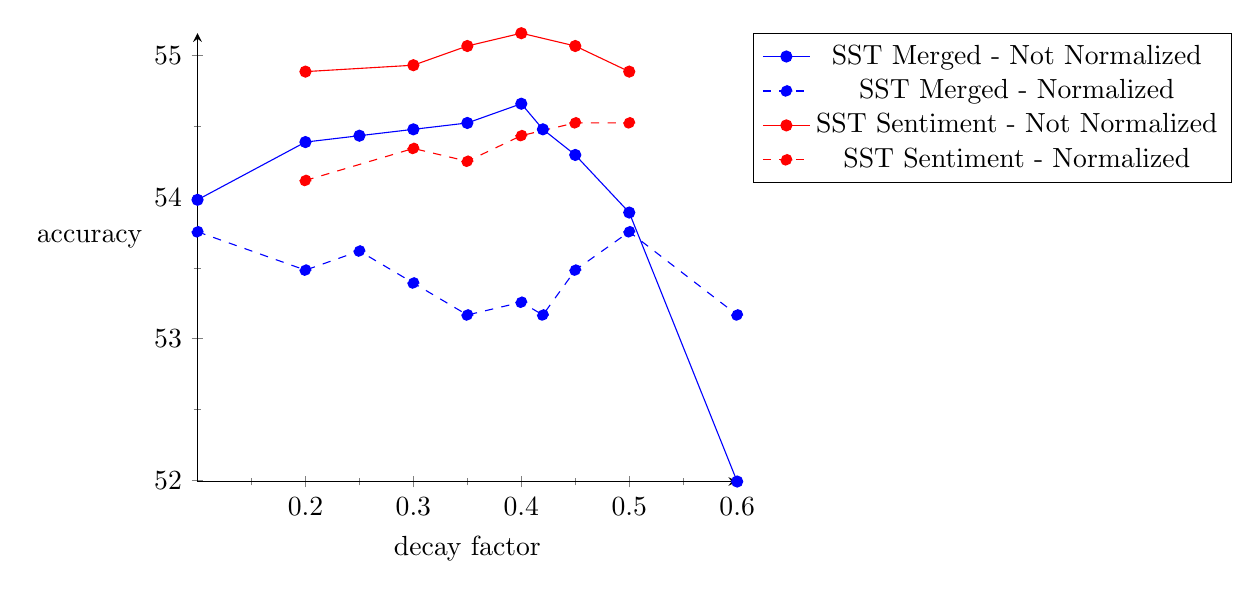
\begin{tikzpicture}
  \begin{axis}[
      axis lines = middle,
      xlabel = decay factor,
      ylabel = accuracy,
      minor tick num = 1,
      legend pos=outer north east,
      xlabel style = {
          at={(axis description cs:0.5,-0.1)},
          anchor=north,
      },
      ylabel style = {
          at={(axis description cs:-0.2,0.5)},
          anchor=south,
      },
  ]
  \addplot[
      color=blue,
      mark=*,
      style=solid,
      ]
      coordinates {
          % (0     , 12.624)           
          (0.1   , 53.981)           
          (0.2   , 54.389)           
          (0.25  , 54.434)           
          (0.3   , 54.479)           
          (0.35  , 54.524)           
          (0.4   , 54.660)
          (0.42  , 54.479)           
          (0.45  , 54.298)           
          (0.5   , 53.891)           
          (0.6   , 51.990)           
      };
      \addlegendentry{SST Merged - Not Normalized}

  \addplot[
      color=blue,
      mark=*,
      style=dashed,
      ]
      coordinates {
          % (0     , 12.624)           
          (0.1   , 53.755)           
          (0.2   , 53.484)           
          (0.25  , 53.619)           
          (0.3   , 53.393)           
          (0.35  , 53.167)           
          (0.4   , 53.257)
          (0.42  , 53.167)           
          (0.45  , 53.484)           
          (0.5   , 53.755)           
          (0.6   , 53.167)           
      };
  \addlegendentry{SST Merged - Normalized}

  \addplot[
      color=red,
      mark=*,
      style=solid,
      ]
      coordinates {
          (0.2, 54.8868778280543)
          (0.3, 54.93212669683258)
          (0.35, 55.067873303167424)
          (0.4, 55.158371040723985)
          (0.45, 55.067873303167424)
          (0.5, 54.8868778280543)
};
  \addlegendentry{SST Sentiment - Not Normalized}

  \addplot[
      color=red,
      mark=*,
      style=dashed,
      ]
      coordinates {
          (0.2, 54.11764705882353)
          (0.3, 54.34389140271493)
          (0.35, 54.25339366515837)
          (0.4, 54.43438914027149)
          (0.45, 54.52488687782805)
          (0.5, 54.52488687782805)
    };
  \addlegendentry{SST Sentiment - Normalized}

  \end{axis}
\end{tikzpicture}
\caption{Confronto degli iperparametri del subset tree kernel.}
\end{figure}

\subsubsection{Subtree Kernel}

\begin{figure}[H]
\centering
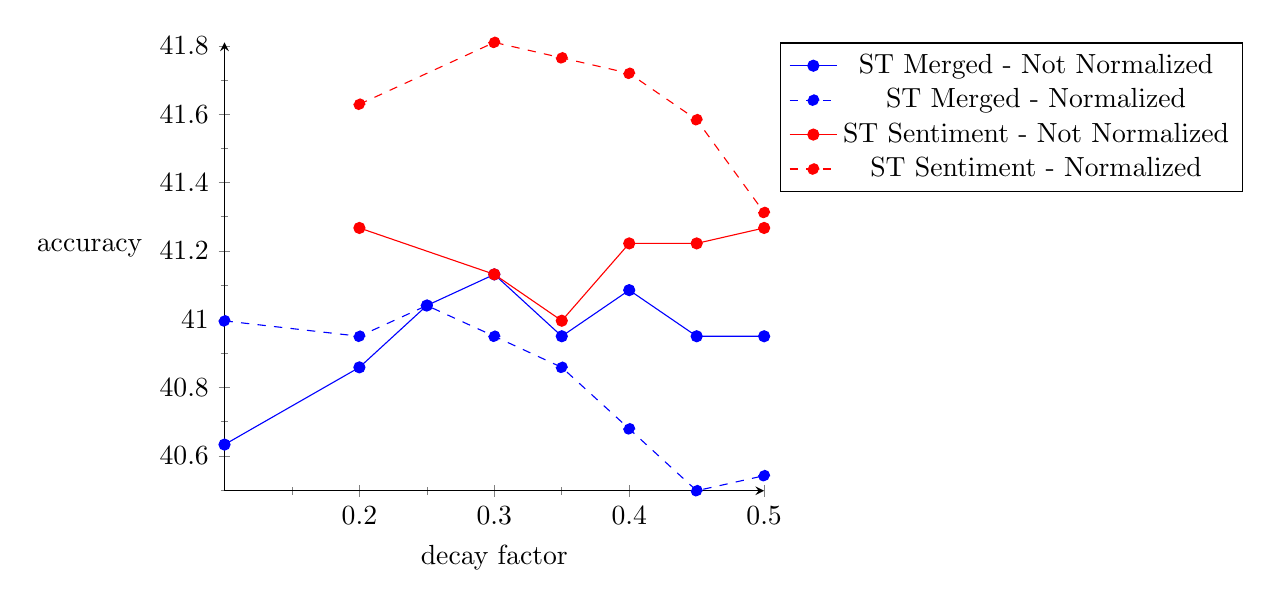
\begin{tikzpicture}
  \begin{axis}[
      axis lines = middle,
      xlabel = decay factor,
      ylabel = accuracy,
      minor tick num = 1,
      legend pos=outer north east,
      xlabel style = {
          at={(axis description cs:0.5,-0.1)},
          anchor=north,
      },
      ylabel style = {
          at={(axis description cs:-0.25,0.5)},
          anchor=south,
      },
  ]
  \addplot[
      color=blue,
      mark=*,
      style=solid,
      ]
      coordinates {
          (0.1   , 40.633)          
          (0.2   , 40.859)          
          (0.25  , 41.040)          
          (0.3   , 41.131)
          (0.35  , 40.950)          
          (0.4   , 41.085)          
          (0.45  , 40.950)          
          (0.5   , 40.950)          
      };
      \addlegendentry{ST Merged - Not Normalized}

  \addplot[
      color=blue,
      mark=*,
      style=dashed,
      ]
      coordinates {
          (0.1   , 40.995)          
          (0.2   , 40.950)          
          (0.25  , 41.040)          
          (0.3   , 40.950)
          (0.35  , 40.859)          
          (0.4   , 40.679)          
          (0.45  , 40.498)          
          (0.5   , 40.542)          

      };
  \addlegendentry{ST Merged - Normalized}


  \addplot[
      color=red,
      mark=*,
      style=solid,
      ]
      coordinates {
            (0.2, 41.26696832579185)
            (0.3, 41.13122171945701)
            (0.35, 40.99547511312217)
            (0.4, 41.22171945701357)
            (0.45, 41.22171945701357)
            (0.5, 41.26696832579185)
    };
  \addlegendentry{ST Sentiment - Not Normalized}

  \addplot[
      color=red,
      mark=*,
      style=dashed,
      ]
      coordinates {
          (0.2, 41.6289592760181)
          (0.3, 41.80995475113122)
          (0.35, 41.76470588235294)
          (0.4, 41.71945701357466)
          (0.45, 41.58371040723982)
          (0.5, 41.31221719457013)
    };
  \addlegendentry{ST Sentiment - Normalized}

  \end{axis}
\end{tikzpicture}
\caption{Confronto degli iperparametri del subtree kernel.}
\end{figure}

\subsubsection{Subset Tree Bow Kernel}

\begin{figure}[H]
\centering
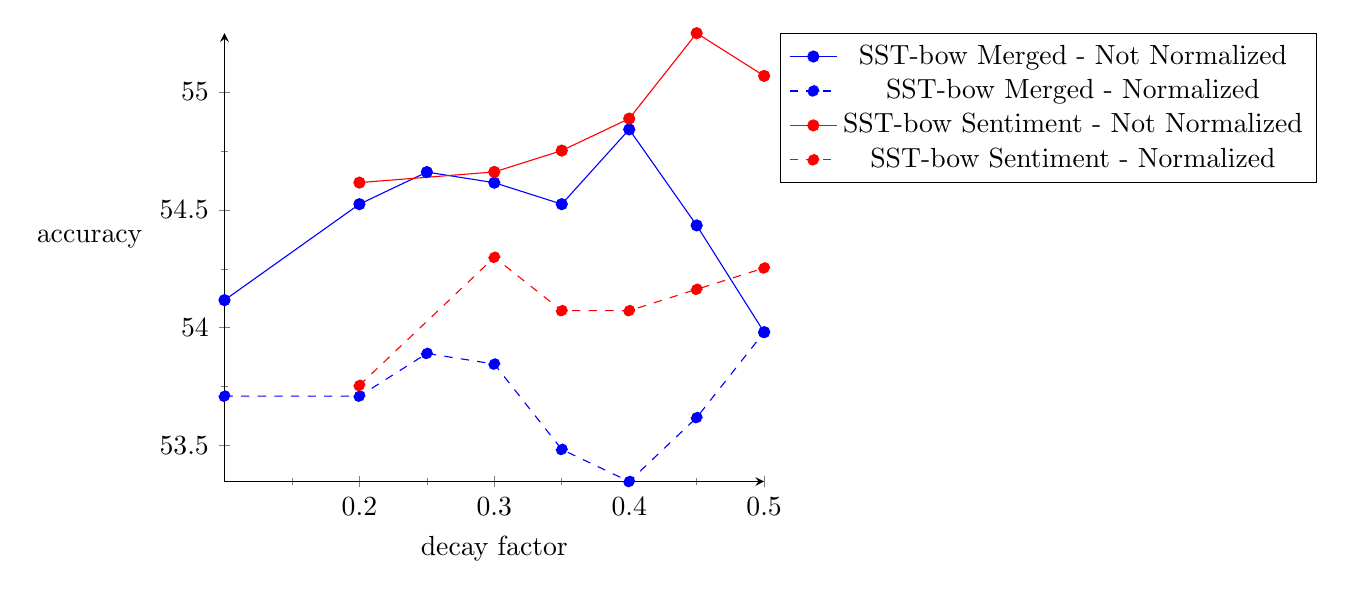
\begin{tikzpicture}
  \begin{axis}[
      axis lines = middle,
      xlabel = decay factor,
      ylabel = accuracy,
      minor tick num = 1,
      legend pos=outer north east,
      xlabel style = {
          at={(axis description cs:0.5,-0.1)},
          anchor=north,
      },
      ylabel style = {
          at={(axis description cs:-0.25,0.5)},
          anchor=south,
      },
  ]
  \addplot[
      color=blue,
      mark=*,
      style=solid,
      ]
      coordinates {
          (0.1       , 54.117)         
          (0.2       , 54.524)         
          (0.25      , 54.660)         
          (0.3       , 54.615)         
          (0.35      , 54.524)         
          (0.4       , 54.841)
          (0.45      , 54.434)         
          (0.5       , 53.981)         
      };
      \addlegendentry{SST-bow Merged - Not Normalized}

  \addplot[
      color=blue,
      mark=*,
      style=dashed,
      ]
      coordinates {
          (0.1   , 53.710)          
          (0.2   , 53.710)          
          (0.25  , 53.891)          
          (0.3   , 53.846)
          (0.35  , 53.484)          
          (0.4   , 53.348)          
          (0.45  , 53.619)          
          (0.5   , 53.981)          

      };
  \addlegendentry{SST-bow Merged - Normalized}

  \addplot[
      color=red,
      mark=*,
      style=solid,
      ]
      coordinates {
        (0.2, 54.61538461538461)
        (0.3, 54.660633484162894)
        (0.35, 54.75113122171946)
        (0.4, 54.8868778280543)
        (0.45, 55.248868778280546)
        (0.5, 55.067873303167424)
};
  \addlegendentry{SST-bow Sentiment - Not Normalized}

  \addplot[
      color=red,
      mark=*,
      style=dashed,
      ]
      coordinates {
        (0.2, 53.755656108597286)
        (0.3, 54.29864253393665)
        (0.35, 54.07239819004525)
        (0.4, 54.07239819004525)
        (0.45, 54.16289592760181)
        (0.5, 54.25339366515837)
    };
  \addlegendentry{SST-bow Sentiment - Normalized}

  \end{axis}
\end{tikzpicture}
\caption{Confronto degli iperparametri del subset tree-bow kernel.}
\end{figure}

\subsubsection{Partial Tree Kernel}

\begin{figure}[H]
\centering
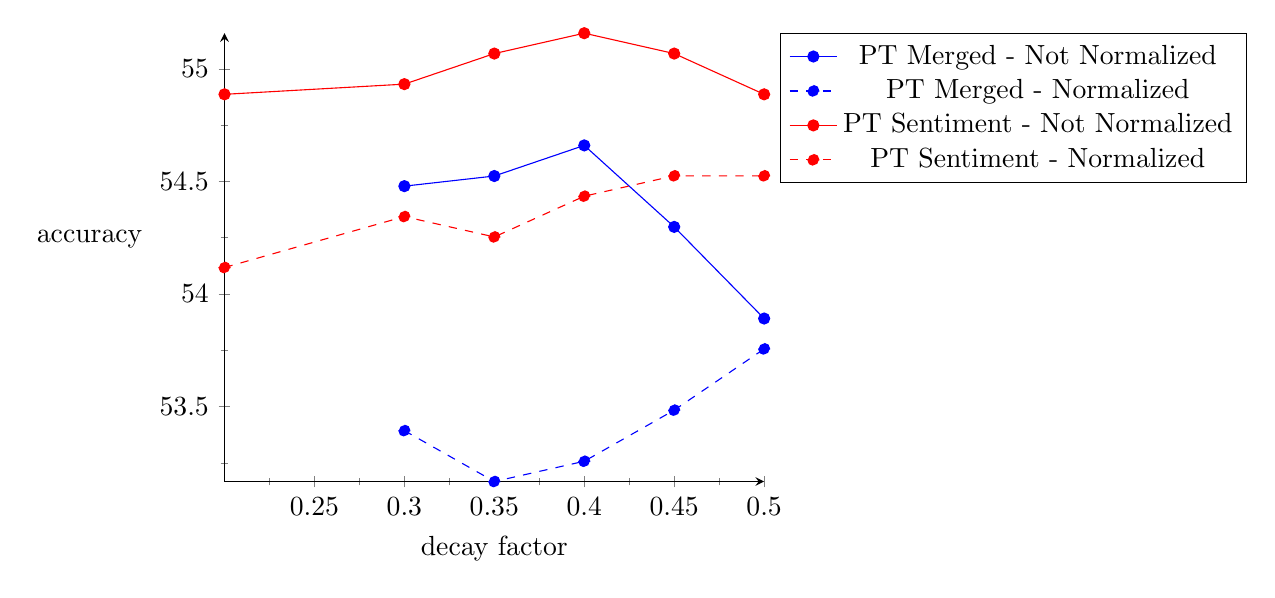
\begin{tikzpicture}
  \begin{axis}[
      axis lines = middle,
      xlabel = decay factor,
      ylabel = accuracy,
      minor tick num = 1,
      legend pos=outer north east,
      xlabel style = {
          at={(axis description cs:0.5,-0.1)},
          anchor=north,
      },
      ylabel style = {
          at={(axis description cs:-0.25,0.5)},
          anchor=south,
      },
  ]
  \addplot[
      color=blue,
      mark=*,
      style=solid,
      ]
      coordinates {
          (0.3       , 54.479)         
          (0.35      , 54.524)         
          (0.4       , 54.660)
          (0.45      , 54.298)         
          (0.5       , 53.891)         
      };
      \addlegendentry{PT Merged - Not Normalized}

  \addplot[
      color=blue,
      mark=*,
      style=dashed,
      ]
      coordinates {
          (0.3       , 53.393)         
          (0.35      , 53.167)         
          (0.4       , 53.257)
          (0.45      , 53.484)         
          (0.5       , 53.756)         
      };
  \addlegendentry{PT Merged - Normalized}


  \addplot[
      color=red,
      mark=*,
      style=solid,
      ]
      coordinates {
        (0.2, 54.8868778280543)
        (0.3, 54.93212669683258)
        (0.35, 55.067873303167424)
        (0.4, 55.158371040723985)
        (0.45, 55.067873303167424)
        (0.5, 54.8868778280543)
      };
  \addlegendentry{PT Sentiment - Not Normalized}

  \addplot[
      color=red,
      mark=*,
      style=dashed,
      ]
      coordinates {
          (0.2, 54.11764705882353)
          (0.3, 54.34389140271493)
          (0.35, 54.25339366515837)
          (0.4, 54.43438914027149)
          (0.45, 54.52488687782805)
          (0.5, 54.52488687782805)
    }
;
  \addlegendentry{PT Sentiment - Normalized}

  \end{axis}
\end{tikzpicture}
\caption{Confronto degli iperparametri del partial tree kernel.}
\end{figure}

\subsubsection{Riassumendo}

\begin{figure}[H]
\centering
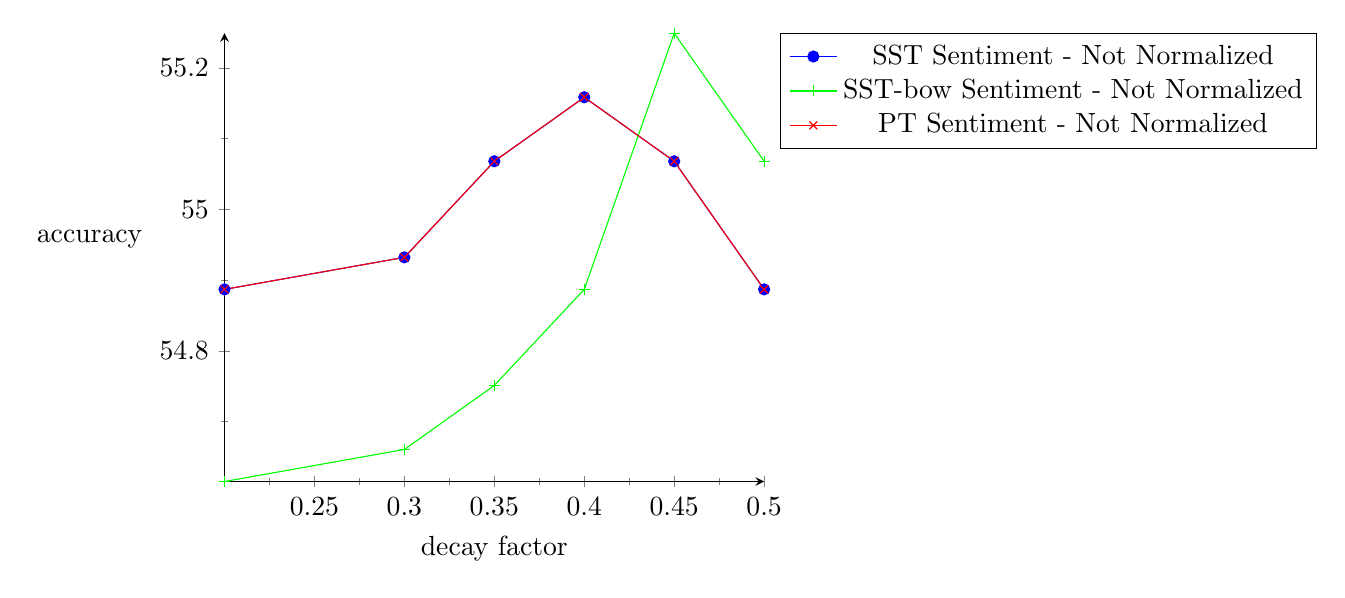
\begin{tikzpicture}
  \begin{axis}[
      axis lines = middle,
      xlabel = decay factor,
      ylabel = accuracy,
      minor tick num = 1,
      legend pos=outer north east,
      xlabel style = {
          at={(axis description cs:0.5,-0.1)},
          anchor=north,
      },
      ylabel style = {
          at={(axis description cs:-0.25,0.5)},
          anchor=south,
      },
  ]

  \addplot[
      color=blue,
      mark=*,
      style=solid,
      ]
      coordinates {
          (0.2, 54.8868778280543)
          (0.3, 54.93212669683258)
          (0.35, 55.067873303167424)
          (0.4, 55.158371040723985)
          (0.45, 55.067873303167424)
          (0.5, 54.8868778280543)
};
  \addlegendentry{SST Sentiment - Not Normalized}

  \addplot[
      color=green,
      mark=+,
      style=solid,
      ]
      coordinates {
        (0.2, 54.61538461538461)
        (0.3, 54.660633484162894)
        (0.35, 54.75113122171946)
        (0.4, 54.8868778280543)
        (0.45, 55.248868778280546)
        (0.5, 55.067873303167424)
};
  \addlegendentry{SST-bow Sentiment - Not Normalized}

  \addplot[
      color=red,
      mark=x,
      style=solid,
      ]
      coordinates {
        (0.2, 54.8868778280543)
        (0.3, 54.93212669683258)
        (0.35, 55.067873303167424)
        (0.4, 55.158371040723985)
        (0.45, 55.067873303167424)
        (0.5, 54.8868778280543)
      };
  \addlegendentry{PT Sentiment - Not Normalized}

  \end{axis}
\end{tikzpicture}
\caption{Confronto dei kernel method sugli iperparametri migliori, si noti che
SST e PT ottengono valutazioni identiche.}
\end{figure}
